\chapter{Statistician's guide} 
\label{chap:stat}

This chapter explains how to write specializing modules. A specializing module is a Python package that defines a PyMC probability model. It needs to expose certain attributes that tell the generic package how to interpret the variables the model contains.

This chapter assumes you know how to use PyMC. See the \href{http://code.google.com/p/pymc/}{PyMC user guide} if you don't.




\section{File structure} 
Try the following from the shell, on a single line:
\begin{verbatim}
    mbg-init-specializing-module duffy-vivax 
        -e 'cut_matern, utils' 
        -a 'Anand Patil, Carlos Guerra, Rosalind Howes'
\end{verbatim}
The command \texttt{mbg-init-specializing-module} is there to help you get the file structure of your specializing module right. It will create Fortran extensions according to the \texttt{-e} option, add the commands to compile them in \texttt{setup.py}, and license the package to the given authors under the GPL. It will also initialize a git repository in the new directory, and make the initial commit.


Take a moment to browse the directory tree you've created, which should look like this:
\begin{center}
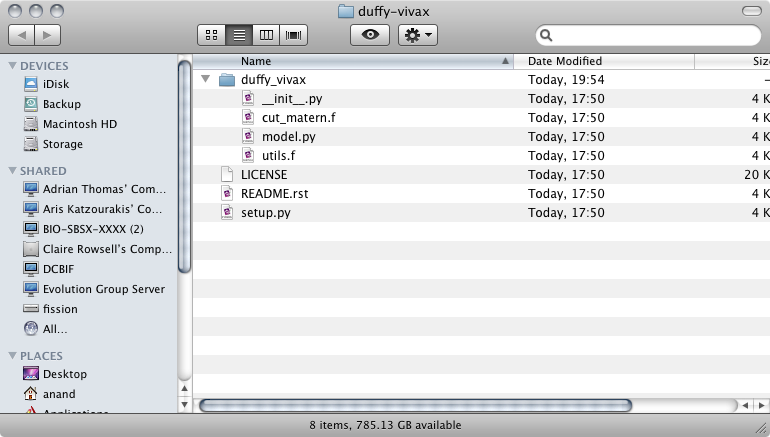
\includegraphics[width=12cm]{filestructure.png}     
\end{center}
Pay special attention to the \texttt{\_\_init\_\_.py} file, which lists the attributes you'll need to define to tell the generic package how to use your specializing module.

\subsection{Importing}
You can install the new package as follows:
\begin{verbatim}
    cd duffy-vivax
    python setup.py develop
\end{verbatim}
See section \ref{sec:spec-local} for more detail. Now change directory to \texttt{\~}, start your favorite Python interpreter, and import the \texttt{duffy\_vivax} module. Browse through its namespace. Pay special attention to the calling conventions of the Fortran subroutines you've generated:
\begin{verbatim}
    In [2]: duffy_vivax.utils.dummy?
    Type:           fortran
    String Form:    <fortran object at 0x1067c4828>
    Namespace:      Interactive
    Docstring:
        dummy - Function signature:
          y = dummy(x)
        Required arguments:
          x : input rank-1 array('d') with bounds (n)
        Return objects:
          y : rank-1 array('d') with bounds (n)
\end{verbatim}
The \texttt{f2py} directives in \texttt{utils.f} (the lines beginning with \texttt{cf2py}) determine which arguments to the subroutine are inputs you need to provide from Python, which inputs Python should see as outputs, and which should be inferred from other arguments. Learning how to write your own Fortran extensions is very worthwhile.

\section{Writing the model}

The primary attribute of a specialization module is a function called \texttt{make\_model}, henceforth the `model factory'. The model factory should take the following arguments:
\begin{description}
    \item[lon] An array of longitudes, in radians.
    \item[lat] An array of latitudes, in radians, of the same length as \texttt{lon}.
    \item[t (optional)] An array of times, in decimal years, of the same length as \texttt{lon}. Spatiotemporal models only.
    \item[covariate\_dict] A dictionary mapping labels to arrays. Each array should give the evaluation of a covariate surface on the \texttt{[lon,lat,t]} input array defined so far.
    \item[**non\_cov\_columns] Any number keyword arguments whose values are arrays of the same length as \texttt{lon}.
\end{description}
These arguments will be read from a user-supplied datafile and fed into the model factory by \texttt{mbg-infer}. The model factory should return its local as follows: 
\begin{verbatim}
    def make_model(lon,lat,covariate_dict,**non_cov_columns):
        ...
        return locals()
\end{verbatim}

\subsection{The fields}

The generic package handles probability models containing one or more Gaussian random fields, whose means are linear combinations of covariate surface evaluations with normally-distributed coefficients, with normally-distributed nuggets:
\begin{equation}
    \label{eq:canonical} 
    \begin{array}{r}
        \beta \stackrel{\textup{\tiny iid}}{\sim} \textup{N}(0,V_{\beta,i}) \\\\
        M:x\rightarrow f_0(x;\phi) + \beta_0 + \sum_{i=1}^n \beta_i c_i(x)\\\\
        C:x,y\rightarrow K(x,y;\theta)\\\\
        f \sim \textup{GP}(M,C)\\\\
        f_x = f(x) \sim \textup{N}(M(x), C(x,x))\\\\
        g_x \sim \textup{N}(f_x, V) 
    \end{array}
\end{equation}
where $K$ is a positive definite covariance function with parameters $\theta$ and $f_0$ is any old function with parameters $\phi$. The generic package does not care what priors you use for $\theta$, $\phi$, $V$ or the $V_\beta$'s, but the coefficients $\beta$ must be iid and normally distributed. Similarly, the package doesn't care how any other variables depend on any of the variables in the model. There may be any number of these Gaussian process submodels in a model.

The nugget and covariates are optional. Without both, the model would be simplified:
\begin{eqnarray*}
    \beta_0\sim\textup{N}(0,V_{\beta,0})\\
    M:x\rightarrow f_0(x;\phi) + \beta_0\\
    C:x,y\rightarrow K(x,y;\theta)\\
    f \sim \textup{GP}(M,C)\\
    f_x = f(x) \sim \textup{N}(M(x), C(x,x))
\end{eqnarray*}

\subsection{Integrating out the covariates}

Using standard multivariate normal transformation rules, the first four lines of model (\ref{eq:canonical}):
\begin{eqnarray*}
    \beta \stackrel{\textup{\tiny iid}}{\sim} \textup{N}(0,V_{\beta,i}) \\
    M:x\rightarrow f_0(x;\phi)+\beta_0 + \sum_{i=1}^n \beta_i c_i(x)\\
    C:x,y\rightarrow K(x,y;\theta)\\
    f \sim \textup{GP}(M,C)
\end{eqnarray*}
can be marginalized to obtain the following model:
\begin{equation}
    \label{eq:int-covariates} 
    \begin{array}{r}
    M:x\rightarrow f_0(x;\phi)\\\\
    C:x,y\rightarrow K(x,y;\theta) + V_{\beta_0} + \sum_{i=1}^n V_{\beta,i}c_i(x)c_i(y)^T\\\\
    f\sim\textup{GP}(M,C)
    \end{array}
\end{equation}
This parameterization is required in the generic package, because experience shows that the MCMC chains tend to mix much better. Section \ref{sub:example} shows how to do this easily. The shell command \texttt{mbg-covariate-traces} can be used to obtain MCMC traces for the $\beta$'s after the MCMC is complete.

\subsection{The nugget and mixing}

The last two lines of model \ref{eq:canonical},
\begin{eqnarray*}
    f_x = f(x) \sim \textup{N}(M(x), C(x,x))\\
    g_x \sim \textup{N}(f_x, V)
\end{eqnarray*}
are slightly nonstandard. Usually, the nugget variance $V$ would be incorporated in the covariance function, and $f_x$ would not be directly imputed. Keeping $f_x$ and $g_x$ separate is strongly recommended in the generic package, however. Experience has shown that the following jumping strategy:
\begin{enumerate}
    \item Metropolis sample each element of $g_x$ one at a time
    \item Gibbs sample $f_x$ jointly conditional on $g_x$
\end{enumerate}
performs well in a wide range of situations. The second step can be performed using the step method \texttt{FieldStepper}, which is provided by the generic package. Section \ref{sub:mcmc-init} describes how to use \texttt{FieldStepper}. 

\subsection{Example field}
\label{sub:example} 

Let's make the submodel in equation \ref{eq:canonical}, reparameterized as in equation \ref{eq:int-covariates}. First, let's make the covariance function and its parameters:
\begin{verbatim}
    amp = pymc.Exponential('amp', .1, value=1.)
    scale = pymc.Exponential('scale_shift', .1, value=.08)
    diff_degree = pymc.Uniform('diff_degree', .01, 1.5)
    
    @pymc.deterministic
    def C(amp=amp, scale=scale, diff_degree=diff_degree):
        return pymc.gp.FullRankCovariance(pm.gp.cov_funs.matern.geo_rad, \
            amp=amp, scale=scale, diff_degree=diff_degree)
\end{verbatim}
Easy enough. Now a trivial mean function:
\begin{verbatim}
    M = pymc.gp.Mean(lamda x: numpy.zeros(x.shape[0]))
\end{verbatim}

Now it gets interesting. The function \texttt{cd\_and\_C\_eval}, provided by the generic package, converts $C$ to the modified covariance function in equation \ref{eq:int-covariates}, with the $V_{\beta,i}$'s set large enough to produce a relatively vague prior, on the practically relevant scale:
\begin{verbatim}
    x = numpy.hstack((lon,lat)).T
    covariate_dict, C_eval = generic_mbg.cd_and_C_eval(covariate_values, C, x)
\end{verbatim}
The output value we're interested in for modelling purposes is \texttt{C\_eval}, but \texttt{covariate\_dict} is important too; the generic package will need to know about it in order to make maps. See section \ref{sub:variable-tags}. Evaluating the mean is more straightforward:
\begin{verbatim}
    M_eval = M(x)
\end{verbatim} 

Now we're ready to create $f_x$ and $g_x$:
\begin{verbatim}
    f_x = pymc.MvNormalCov('f_x', M_eval, C_eval)
    g_x = pymc.Normal('g_x', 1/V)
\end{verbatim}
PyMC parameterizes the normal distribution by precision rather than variance, so the second parameter of $g_x$ is $\tau=1/V$. That's all there is to producing GP submodels in the generic package. You can complete the model any way you like: add more GP submodels, likelihoods, etc.

\subsection{Be sure to commit}
\label{sub:git-commit} 
It's important to commit any changes you make to the specialization module to the local repository before running any MCMC, because the hash of the current git head is stored in the MCMC trace. If the state of the code doesn't correspond to the hash, you may not be able to reproduce your results later.

\section{Required attributes}

The specialization module needs to expose several attributes in addition to \texttt{make\_model}. See \texttt{\_\_init\_\_.py} in the package you just created, \texttt{duffy\_vivax}

\subsection{Metadata and non-covariate columns}
\subsubsection{Non-covariate columns} 
The attribute \texttt{non\_cov\_columns} is a dictionary mapping labels to type strings (such as \texttt{'float'}, \texttt{'int'}, \texttt{'str'}, etc.). The generic package will expect to find the labels as column headers in any CSV datafiles provided by the end user. 
\subsubsection{Arbitrary metadata} 
The attribute \texttt{metadata\_keys} allows you to store any local variable generated by the model factory in the trace. If your \texttt{metadata\_keys} are \texttt{['n\_tacos', 'fillings']}, then the corresponding variables can be retrieved from the trace file using \texttt{hf.root.metadata.n\_tacos[0]}, etc.

\subsection{Tagging the Gaussian process submodels}
\label{sub:variable-tags} 
The following attributes tag certain variables created by the model factory as playing certain roles in GP submodels:
\begin{description}
    \item[\texttt{f\_labels}] A list giving the names of the variables that represent field evaluations. For the submodel in section \ref{sub:example}, you could use either \texttt{['f\_x']} or \texttt{['g\_x']}. It's completely up to you and shouldn't make much difference at any stage.
    \item[\texttt{fs\_have\_nugget}] A dictionary mapping the \texttt{f\_labels} to booleans indicating whether they have a nugget variance. In the context of \ref{sub:example}, you would use either \texttt{\{'f\_x': False\}} or \texttt{\{'g\_x': True\}}, depending on which \texttt{f\_label} you chose.
    \item[\texttt{nugget\_labels}] A dictionary mapping the \texttt{f\_labels} to the labels of their associated nugget variances, ie \texttt{\{'f\_x': 'V'\}}. Not used at keys where \texttt{fs\_have\_nugget} is false.
    \item[\texttt{M\_labels}, \texttt{C\_labels}]: Dictionaries mapping the field labels to the labels of their corresponding means and covariances. For section \ref{sub:example}, these would be \texttt{\{'g\_x': 'M'\}} and \texttt{\{'g\_x': 'C'\}}, assuming you chose $g_x$ as the field label.
    \item[\texttt{x\_labels}]: A dictionary mapping the field labels to the array of input locations on which the field was evaluated, ie \texttt{\{'f\_x': 'x'\}}.
    \item[\texttt{diags\_safe}]: Some covariance functions have parameters called \texttt{amp}, and have the property
    \begin{verbatim}
        numpy.all(C.params['amp']**2==numpy.diag(C(x,x)))
    \end{verbatim}
The \texttt{diags\_safe} attribute is a dictionary mapping the field labels to booleans indicating whether this property holds for their associated covariance functions.
\end{description}

\subsection{Postprocessing functions}

\subsubsection{Postprocessing for map generation}
The specialization package must expose a function called \texttt{map\_postproc}. It should take arguments corresponding to all of the \texttt{f\_labels}, which will be field evaluations of arbitrary shape, and return... whatever it is you want to show the per-pixel predictive distribution of in the maps. For example, if your model is a spatial GLM with count data and an inverse-logit link function, this function would do:
\begin{verbatim}
    def map_postproc(g_x):
        return generic_mbg.invlogit(g_x)
\end{verbatim}
The generic package's link functions should be preferred to all others when possible, because they're multithreaded.

The map postprocessing function can take initial arguments corresponding to tallied variables in the probability model. For example, if you wanted to use Stukel's link function, and had shape variables $a_1$ and $a_2$ in the model:
\begin{verbatim}
    def map_postproc(g_x, a1, a2):
        return generic_mbg.stukel_invlogit(g_x, a1, a2)
\end{verbatim}

\subsubsection{Postprocessing for validation} 
When validating, the postprocessing function may need to take into account some aspects of the held-out dataset. For that reason, \texttt{validate\_postproc} must take keyword arguments corresponding to the non-covariate columns, and it must return a function with the same calling convention as \texttt{map\_postproc}. The shell command \texttt{mbg-validate} will read the non-covariate columns from the held-out datasheet, pass them into \texttt{validate\_postproc}, and use the returned function to convert the Gaussian field realizations to predictions.

\subsection{Initializing the MCMC object}
\label{sub:mcmc-init} 

The shell command \texttt{mbg-infer} will call \texttt{make\_model} and wrap the jumble of variables it returns in a PyMC \texttt{MCMC} object. Before it begins sampling, it will call \texttt{mcmc\_init} on the MCMC object. This is your chance to assign custom step methods, etc. For example, to use the generic package's \texttt{FieldStepper} on the Gaussian field evaluation in section \ref{sub:example}:
\begin{verbatim}
    def mcmc_init(M):
        M.use_step_method(generic_mbg.FieldStepper, \
            M.f_x, M.V, M.C_eval, M.M_eval, M.x, M.g_x)
\end{verbatim}
